\documentclass[12pt, a4paper, twocolumn]{report}
\usepackage[utf8]{inputenc}
\usepackage[russian]{babel}
\usepackage{hyperref}
\usepackage[]{graphicx}

%\makeindex

\newcommand{\IMPORTANT}{

{\bf ВНИМАНИЕ:~}}

\newcommand{\PARAM}[1]{\item {\bf #1} }
\newcommand{\PARAMSECTION}[1]{\vbox{}{\bf Раздел <<#1>>}}

\title{Установка №~4 для измерения удельного сопротивления при постоянной температуре. Руководство пользователя}
\author{Накин~А.~В.}

\begin{document}

\maketitle

\tableofcontents

\chapter{Общие сведения}

Установка №~4 (далее~--- Установка) представляет собой программно-аппаратный комплекс для измерения удельного сопротивления низкоомных материалов (далее~--- Образцов) при постоянной температуре.

Установка производит съём показаний измерительных приборов, вычисление значения сопротивления со всеми сопутствующими погрешностями и запись результатов в файл. В зависимости от конфигурации Установка может регулировать ток питания в указанном диапазоне, таким образом измеряя зависимость сопротивления Образца от тока.

Установка не управляет температурой Образца и не измеряет её.

\section{Состав Установки}

\subsection{Состав аппаратной части}

Аппаратная часть Установки состоит из следующих приборов.

\begin{itemize}

\item Мультиметр 34410A компании Agilent (2~шт.). Предназначен для измерения падения напряжения на Образце и силы тока в цепи.

\item Управляемый источник питания постоянного тока (далее~--- ИП) E3645A компании Agilent (0-1~шт.). Предназначен для подачи тока в цепь с Образцом. Управляется ПЭВМ и позволяет автоматизированное измерение сопротивления в диапазоне токов. В зависимости от конфигурации Установки может отсутствовать.

\item Произвольный неуправляемый ИП постоянного тока (0-1~шт.). Предназначен для подачи тока в цепь с Образцом. Используется вместо E3645A в тех случах, когда требуется повышенная стабильность тока питания и не требуется измерение сопротивления в диапазоне токов.

\item Блок из 8-ми управляемых 2-х позиционных реле МВУ-8 компании ОВЕН (1~шт.). Предназначен для коммутации приборов и Образца. Управляется ПЭВМ посредством прибора АС-4.

\item Преобразователь интерфейсов USB/RS-485 АС-4 компании ОВЕН (1~шт.). Предназначен для подключения МВУ-8 к ПЭВМ через USB интерфейс.

\item Эталонное сопротивление (0-1~шт.). Предназначено для измерения тока в цепи посредством измерения падения напряжения на сопротивлении с известным номиналом. В зависимости от конфигурации Установки может отсутствовать, тогда ток в цепи измеряется мультиметром 34410A, работающим в режиме амперметра.

\end{itemize}

\subsection{Состав программной части}
\label{sec_software}

Программная часть Установки состоит из следующих компонентов.

\begin{itemize}

\item Программа Установки, состоящая из нескольких модулей, написанных на языке Tcl.

\item Интерпретатор языка Tcl и необходимые библиотеки.

\item Библиотека, предоставляющая программный интерфейс VISA для доступа к приборам 34410A и E3645A.

\item Драйвер устройства АС-4, представляющий устройство в виде COM-порта.

Сведения об установке интерпретатора Tcl, библиотек для него, библиотеки VISA изложены в соответствующих документах. Сведения об установке драйвера АС-4 см. в документации к прибору или на сайте производителя\footnote{\href{http://www.owen.ru/}{http://www.owen.ru/}}.

\end{itemize}

\section{Принцип работы}

В цепь с источником постоянного тока последовательно включён Образец, чьё сопротивление нужно измерить. Установка одновременно измеряет падение напряжение на образце и ток в цепи, по которым вычисляет сопротивление образца.

Установка может менять силу тока в заданном интервале, таким образом измеряя зависимось сопротивления Образца от величины протекающего через него тока.

Для устранения постоянных составляющих в погрешности измерения Установка может производить т.~н. <<переполюсовки>>, то есть менять полярность подключения как вольтметра, так и источника тока, и объединять результаты измерений. 

\section{Режимы работы}

\subsection{Управление питанием}

Установка может работать в одном из двух режимов управления питанием: ручном и автоматизированном.

\subsubsection{Автоматизированное управление}
\label{sec_auto_current}

Данный режим используется в случае, когда необходимо получить токовую зависимость сопротивления Образца в некотором интервале токов. Интервал изменения тока и шаг приращения вводятся оператором перед началом измерений. Для каждого значения тока производится измерение сопротивления, результаты записываются в файл.

В данном режиме Установка управляет током в цепи посредством ИП E3645A.

\subsubsection{Ручное управление}
\label{sec_manual_current}

Данный режим используется, когда стабильность в цепи тока, предоставляемая E3645A, недостаточна и вносит серьёзную погрешность в измерения сопротивления. В этом случае в цепь включается произвольный источник питания, управляемый вручную оператором.

В данном режиме Установка не управляет током в цепи, а производит однократное измерение сопротивления и записывает результаты в файл. Далее оператор может вручную изменить ток в цепи и повторить измерение.

\subsection{Способ измерения тока}

Установка может измерять ток в цепи двумя способами: непосредственно при помощи амперметра и путём измерения падения напряжения на эталонном сопротивлении. Правильное подключение мультиметра для каждого из режимов производится при помощи блока реле МВУ-8.

\subsubsection{Непосредственное измерение}
\label{sec_direct_measure}

В данном режиме мультиметр №~2 работает как амперметр и включён последовательно в цепь с образцом. Эталонное сопротивление не используется.

Преимущества:

\begin{itemize}
\item Не требуется эталонное сопротивление.
\item Измерения дают <<истинное>> значение сопротивления, которое не зависит от точности номинала эталонного сопротивления.
\end{itemize}

Недостатки:

\begin{itemize}
\item Точность измерения постоянного тока мультиметром Agilent 34410A примерно в 10~раз ниже точности измерения постоянного напряжения. Если в эксперименте важна не абсолютная, а относительная (относительно предыдущих измерений) точность, рекомендуется измерение тока посредством эталонного сопротивления.
\end{itemize}

\subsubsection{Измерение падения напряжения}
\label{sec_test_measure}

В данном режиме в цепь последовательно с образцом включено эталонное сопротивление известного номинала, а мультиметр №~2 работает как вольтметр и измеряет падение напряжения на эталоне.

Преимущества:

\begin{itemize}
\item Поскольку постоянное напряжение измеряется с меньшей инструментальной погрешностью, чем постоянный ток, этот метод может дать лучшую точность в <<относительных>> измерениях, когда сравниваются результаты нескольких измерений над одной и той же серией образцов, например до и после облучения.
\end{itemize}

Недостатки:

\begin{itemize}
\item От оператора требуется обеспечивать стабильность величины эталонного сопротивления в разных сериях измерений, которые могут производиться в различных условиях, например при значительных колебаниях температуры в лаборатории.
\item Точность определения <<истинного>> значения сопротивления образца напрямую зависит от точности номинала эталонного сопротивления. В большинстве случае более точное истинное значение может быть получено в методе непосредственного измерения тока мультиметром.
\end{itemize}

\section{Принципиальная схема}

Принципиальная схема Установки приведена на рис.~\ref{pic-scheme}.

Мультиметры PV1, PV2, ИП I1 и эталонное сопротивление R2 подключаются к выходам разъёма J1. К разъёму J2 подключён Образец R1.

Мультиметр PV1 работает как вольтметр и измеряет падение напряжения на Образце. Он подключается посредством сдвоенного переключателя S1, при помощи которого меняется полярность подключения вольтметра.

ИП I1 подключён к схеме посредством сдвоенного переключателя S2, при помощи которого меняется полярность питания цепи.

Мультиметр PV2 работает либо как вольтметр, если используется эталонное сопротивление, либо как амперметр для непосредственного измерения силы тока в цепи.

Сдвоенный переключатель S3 подключает или отключает эталонное сопротивление в зависимости от режима работы Установки. В положении, изображённом на схеме, эталонное сопротивление подключено.

Переключатель S4 предназначен для кратковременного размыкания цепи во время измерения полярности переключателями S1 или S2. Размыкание необходимо для того, чтобы избежать закорачивания выходов источника питания. В положении, изображённом на схеме, цепь замкнута.

Конструкционно переключатели S1-S4 размещены в одном блоке реле МВУ-8.

\begin{figure*}
\begin{center}
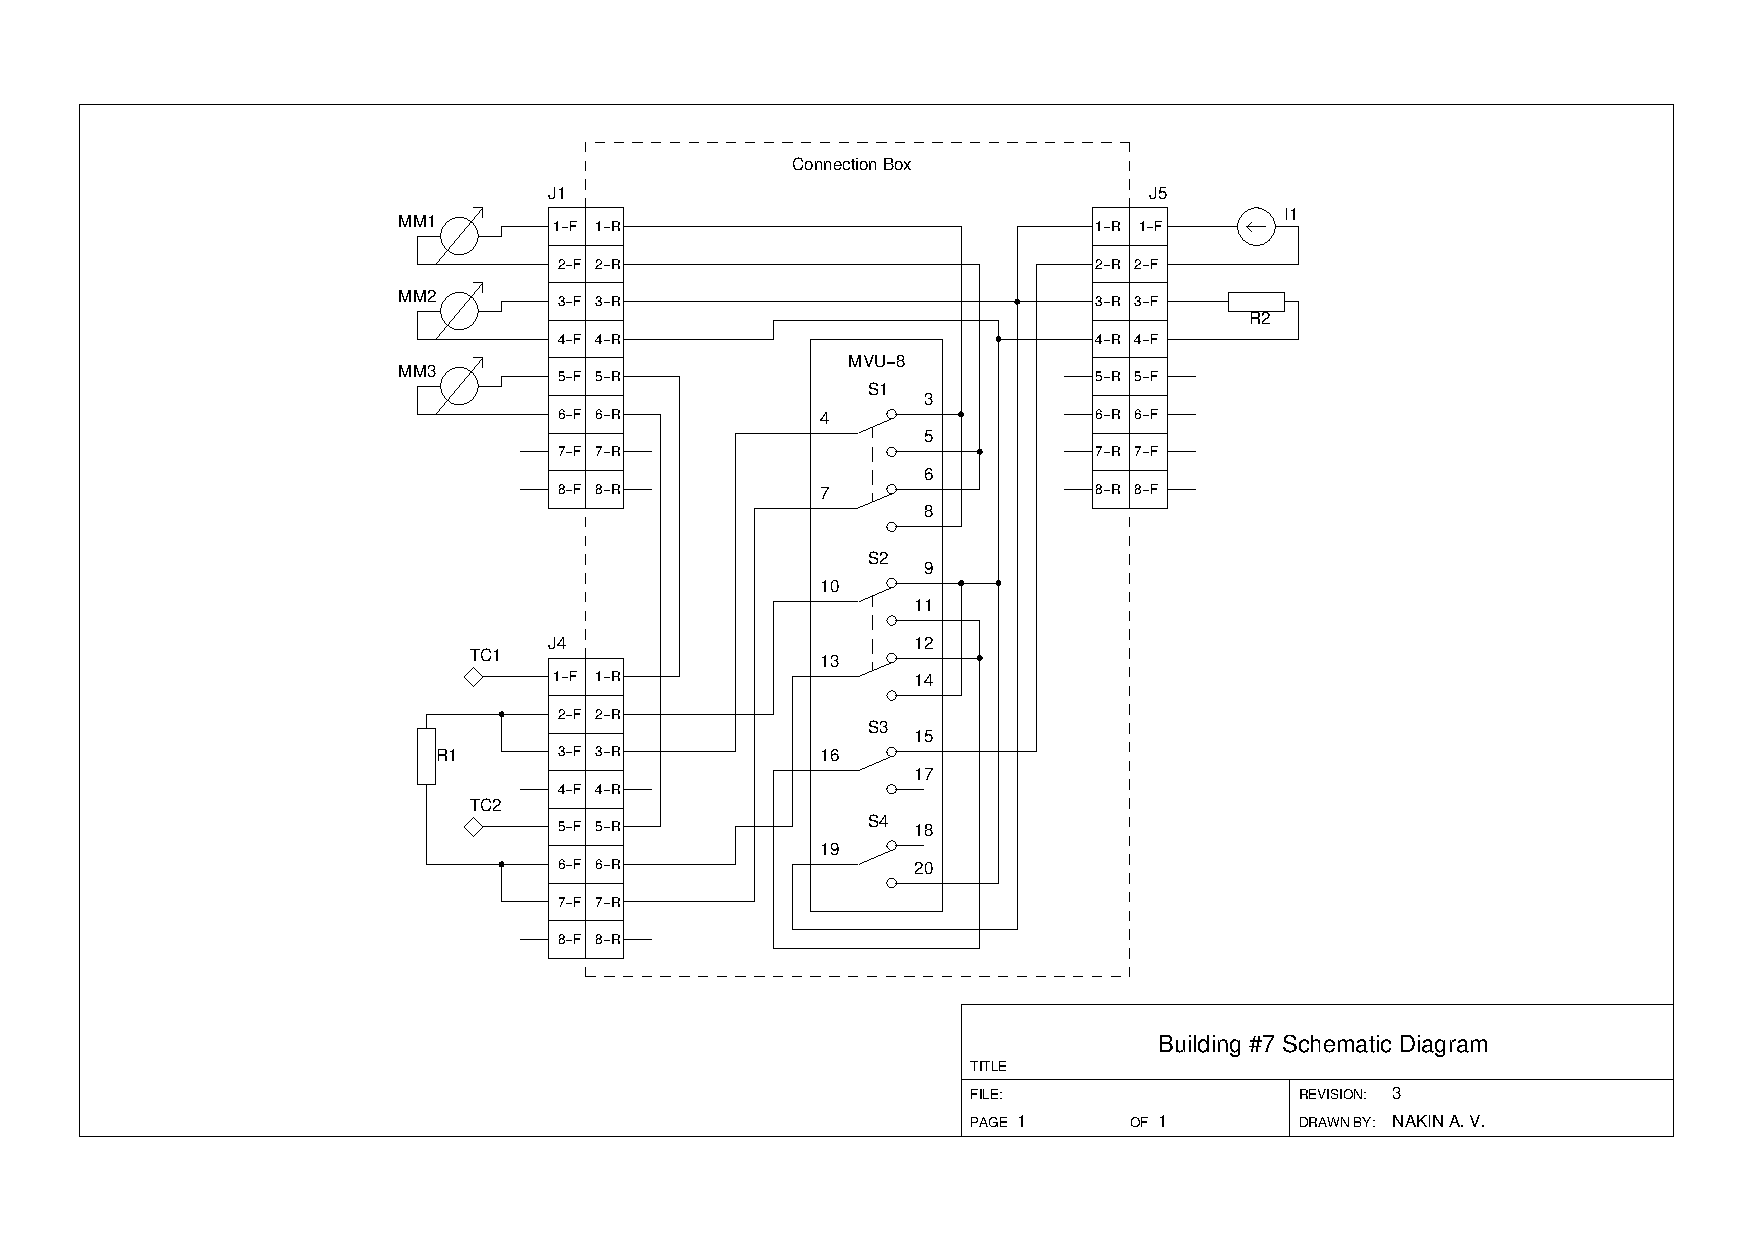
\includegraphics[width=1.0\textwidth, clip, viewport=50 60 450 540]{scheme}
%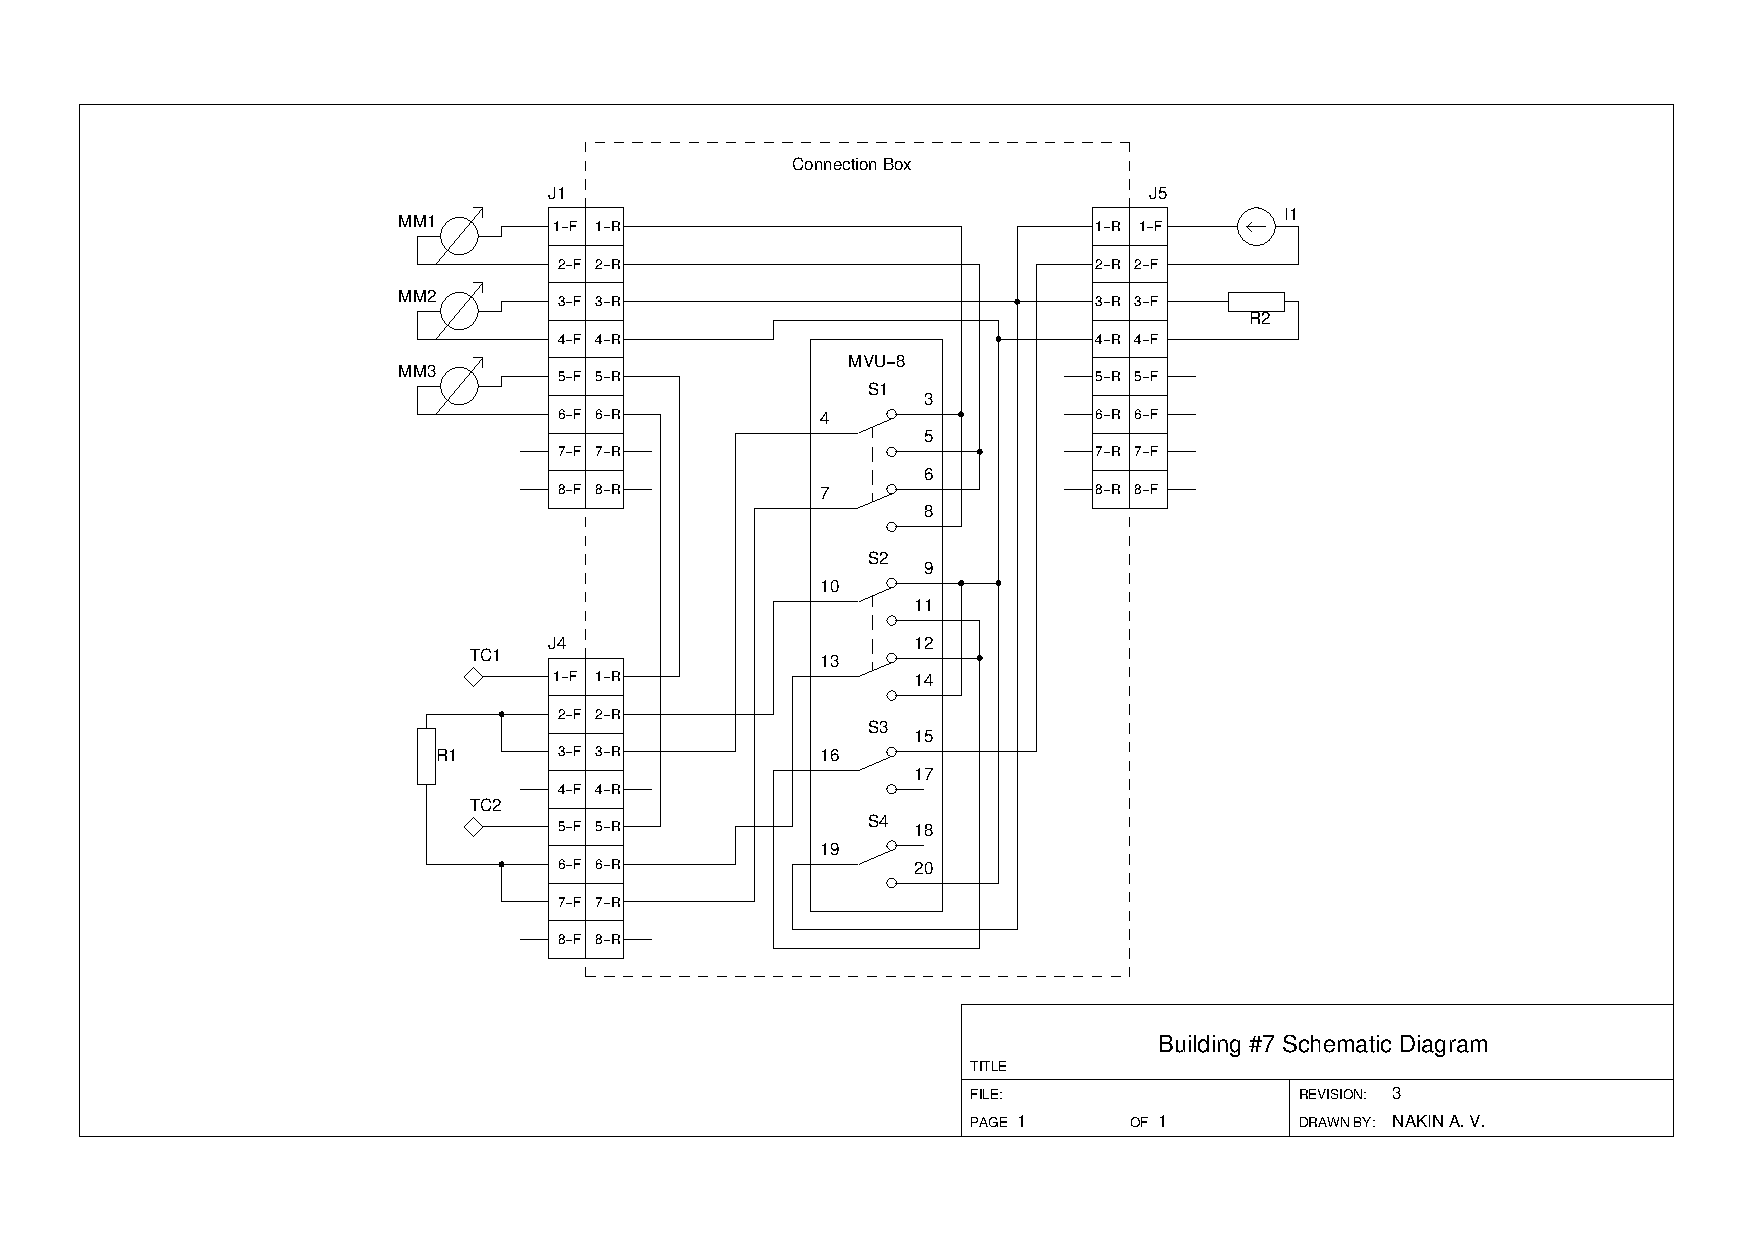
\includegraphics[width=0.9\textwidth, clip, viewport=0 655 600 785]{scheme}
\end{center}
\caption{Принципиальная схема Установки}
\label{pic-scheme}
\end{figure*}

\chapter{Подготовка к работе}

\section{Подготовка аппаратной части}

\subsection{Подготовка мультиметров 34410A}

Мультметры должны быть включены и подключены к ПЭВМ посредством интерфейса USB.

Выходы первого мультиметра должны быть установлены в положение для измерения напряжения

Если Установка сконфигурирована для измерения тока в цепи посредством непосредственного измерения, выходы второго мультиметра должны быть установлены в положение для измерения тока. В противном случае выходы должны быть установлены в положение для измерения напряжения.

\subsection{Подготовка ИП E3645A}

ИП должен быть включен и подключён к ПЭВМ посредством интерфейса RS-232. Выходы ИП должны быть подключены к соответствующим разъёмам Установки.

ИП должен быть настроен для работы по интерфейсу RS-232. Согласно настройкам по умолчанию (<<заводским>>) он работает по интерфейсу GPIB. В этом случае прибор требует перенастройки на использование RS-232. Изменённые настройки сохраняются в энергонезависимой памяти устройства и не теряются при выключении питания. См. документацию к Agilent E3645A для детальных инструкций.

\subsection{Подготовка МВУ-8}

Устройство должно быть включено и подключено к сети RS-485, управляемой АС-4.

Устройство должно быть настроено на работу по протоколу <<Modbus RTU>>. Согласно <<заводским>> настройкам устройство использует протокол <<ОВЕН>>. Для смены протокола необходимо запустить программу <<Конфигуратор МВУ-8>> и в ней перенастроить устройство. Настройки сохраняются в энергонезависимой памяти и не теряются при выключении питания. См. документацию к программе для детальных инструкций.

\IMPORTANT Всякий раз при запуске программы <<Конфигуратор МВУ-8>> МВУ-8 автоматически переходит на протокол <<ОВЕН>>. Чтобы вернуть устройство на нужный протокол, нужно выключить его на несколько секунд и включить снова.

\subsection{Подготовка АС-4}

Устройство должно быть подключено к ПЭВМ посредством интерфейса USB. Если драйвер корректно установлен, в системе должен появиться новый COM-порт, посредством которого программы взаимодействуют с устройствами в сети RS-485.

\section{Подготовка программной части}

Подготовка программной части сводится к установке всех необходимых программных компонентов (см. раздел <<\hyperref[sec_software]{Состав программной части}>>) и настройке программы Установки.

Установка программных компонентов рассмотрена в соответствующих документах.

Для настройки параметров программы Установки (далее~--- Программы) необходимо её запустить.

\subsection{Запуск Программы}

Для запуска Программы наберите команду следующего вида:

{\small
\begin{verbatim}
 wish85 -encoding utf-8 assembly004.tcl
\end{verbatim}
}

Здесь {\tt wish85}~--- название программы-интерпретатора Tcl версии 8.5 (версия, а значит и название может отличаться); {\tt assembly004.tcl}~--- имя главного модуля Программы.

Рекомендуется настроить операционную систему таким образом, чтобы запуск любой программы, написанной на Tcl и имеющей расширение {\tt .tcl} можно было осуществлять просто кликом по ней из менеджера файлов.

Если все необходимые программные компоненты присутствуют и правильно настроены, откроется окно Программы.

\subsection{Настройка параметров программы}

Все параметры Программы условно делятся на две части:

\begin{itemize}

\item \emph{Параметры установки}: параметры, которые не требуют частого изменения, такие как адреса устройств. Как правило, эти параметры, будучи настроенными, не требуют изменения до тех пор, пока не изменится конфигурация устройств Установки.

\item \emph{Параметры измерения}: параметры, влияющие на процесс измерения. Как правило, эти параметры требуют подстройки перед каждым сеансом работы Установки.

\end{itemize}

\subsubsection{Параметры установки}

Ниже приведены параметры установки. Все поля обязательны для заполнения, если не оговорено обратное.

\begin{itemize}

\PARAM{Порт для АС-4}

COM-порт, направленный на нужный экземпляр АС-4. 

\PARAM{Сетевой адрес МВУ-8}

МВУ-8, как и всякое устройство в сети RS-485, имеет уникальный внути сегмента сети 8-ми битный адрес, представленный целым десятичным числом. Как правило, он написан на самом устройстве МВУ-8. Чтобы узнать и, при необходимости, изменить адрес запустите программу <<Конфигуратор МВУ-8>>.

\PARAM{VISA адрес источника питания}

VISA-адрес ИП E3645A. Если в Установке используется ручное управление питанием, можно оставить это поле пустым.

\PARAM{VISA адрес вольтметра на образце}

VISA-адрес мультиметра 34410A, работающего в режиме вольметра и измеряющего напряжение на Образце.

\PARAM{VISA адрес вольтметра на эталоне}

VISA-адрес мультиметра 34410A, работающего в режиме вольметра и измеряющего напряжение на эталонном сопротивлении (если оно используется в Установке), или же в режиме амперметра и измеряющего непосредственно ток в цепи.

\PARAM{Звуковой сигнал по окончании}

Если данный флажок отмечен, по окончании измерений один из мультиметров подаст короткий звуковой сигнал.

\end{itemize}

\subsubsection{Параметры измерения}

Ниже приведены параметры измерения. В зависимости от конфигурации Установки часть полей может быть <<запрещена>>, то есть недоступна для редактирования. Все остальные поля обязательны для заполнения, если не оговорено обратное.

\PARAMSECTION{Питание образца}

\begin{itemize}

\PARAM{Ручное управление}

Если данный флажок отмечен, Установка работает в режиме ручного управления питанием. При этом поля для ввода диапазона изменения тока запрещены.

\PARAM{Начальный ток}

В автоматизированном режиме управления питанием это поле определяет начальный ток, то есть ток, при котором будет произведено первое измерение.

\PARAM{Конечный ток}

В автоматизированном режиме управления питанием это поле определяет конечный ток, то есть ток, при котором будет произведено последнее измерение. Значение должно быть больше или равно значению начального тока.

\PARAM{Приращение}

В автоматизированном режиме управления питанием это поле определяет изменение тока на каждом шаге.

\PARAMSECTION{Параметры измерения}

\PARAM{Циклов 50 Гц на измерение}

Для уменьшения погрешности мультиметры производят многократные измерения в течении некоторого времени, после чего возвращают усреднённое значение в качестве результата. Поскольку основным источником шумов является переменный ток сети питания, периоды измерения привязаны к периодам колебаний тока в сети. В документации к мультиметру Agilent 34410A этот параметр называется NPLC (Number of Power Line Cycles~--- число циклов линии питания). В наших условиях частота сети равна 50~Гц, следовательно каждый цикл имеет продолжительность 20~мс.

Для того, чтобы свести эффект влияния шумов  линии питания к минимум, данный параметр должен иметь целое значение. Рекомендуемое значение параметра~--- 10, в этом случае каждое измерение производится в течении 200~мс.

\PARAM{Измерений на точку}

Установка может производить многократные измерения при одном и том же токе, после чего вычислять и сохранять среднее значение в качестве результата. Разброс значений будет учитываться при вычислении погрешности измерений.

Минимальное значение параметра~--- 1. Если позволяют условия эксперимента, рекомендуется производить не менее 100 измерений.

Время измерения зависит от величины параметров <<Циклов 50 Гц на измерение>> и <<Измерений на точку>>. Например, если первый параметр имеет значение 10, а второй~--- 100, то каждая точка результирующей зависимости будет измеряться в течении $0,02 \cdot 10 \cdot 100 = 20$~секунд (здесь $0,02$~--- продолжительность одного периода колебаний напряжения в сети). При использовании переполюсовок продолжительность измерения увеличивается в 2 (при переполюсовке напряжения \emph{или} тока) или в 4 (при переполюсовке и напряжения и тока) раза.

\PARAM{Игнорировать инстр. погрешность}

В некоторых случаях может потребоваться исключить из результирующей ошибки измерения сопротивления инструментальную погрешность. В этом случае флажок должен быть отмечен.

При отключённой инструментальной погрешности ошибкой измерения является стандартное отклонение величины сопротивления в результате нескольких измерений (количество которых определяет параметром <<Измерений на точку>>).

\PARAMSECTION{Метод измерения тока}

\PARAM{Амперметром}

Если флажок отмечен, сила тока измеряется непосредственно амперметром.

\PARAM{Напряжением на эталоне}

Если флажок отмечен, сила тока измеряется через падение напряжение на эталонном сопротивлении.

\PARAM{Эталонное сопротивление}

В данном поле вводится величина эталонного сопротивления, которое используется для измерения силы тока в цепи.

\PARAMSECTION{Переполюсовки}

\PARAM{Переполюсовка напряжения}

Если флажок отмечен, Установка в процессе измерения производит переключение полярности подключения вольтметра к Образцу.

\PARAM{Переполюсовка тока}

Если флажок отмечен, Установка в процессе измерения производит переключение полярности подключения ИП.

\PARAMSECTION{Файл результатов}

\PARAM{Имя файла}

Имя файла, куда будут сохраняться результаты измерения. Если поле пусто, запись в файл не производится.

\PARAM{Формат файла}

Формат результирующего файла. Может иметь следующие значения:

\begin{itemize}
\item TXT~--- каждое измерение занимает одну строку, значения в строке разделены символом табуляции (09h). Комментарием считается строка, начинающаяся с символа <<\#>>.
\item CSV~--- каждое измерение занимает одну строку, значения в строке разделены запятой. Первая строка является комментарием. Файлы данного формата удобны для открытия в программе MS~Excel и аналогах.
\end{itemize}

\PARAM{Переписать файл}

Если флажок отмечен, в начале измерений предыдущее содержимое файла уничтожается. Такой режим удобен при автоматизированном управлении током в цепи.

Если флажок сброшен, результаты будут добавляться в конец файла без его перезаписи. Такой режим удобен при ручном управлении питанием.

\end{itemize}

\end{document}
